\documentclass[11pt,a4paper]{article}

\usepackage[a4paper,margin=1in]{geometry}
\usepackage[T1]{fontenc}
\usepackage[utf8]{inputenc}
\usepackage{lmodern}
\usepackage{setspace}
\usepackage{hyperref}
\usepackage{xurl}
\usepackage{microtype}
\usepackage{graphicx}

\setstretch{1.0}
\urlstyle{tt}
\emergencystretch=2em

\title{Software Development Report}
\author{Brandon MacGillivray}
\date{\today}

\begin{document}

\hypersetup{pageanchor=false}
\begin{titlepage}
\centering
{\LARGE Software Development Report\par}
\vspace{1.5cm}
{\large An investigation into Lightweight Hand Pose estimation for Edge HCI\par}
\vspace{1cm}
{\large Brandon MacGillivray\par}
\vspace{0.5cm}
{\large 40321491\par}
\vfill
\end{titlepage}
\hypersetup{pageanchor=true}

\section*{Acknowledgements}

\tableofcontents
\newpage

\section{Purpose, Operation and Validation}

The software is intended to implement and evaluate a lightweight 2D hand pose estimation pipeline for edge HCI, with a DRHand-inspired dual-branch model that predicts hand keypoints from RGB images and supports training, inference, benchmarking, and reproducible experiment reruns.

\medskip

\noindent The source repository for this software is available at
\url{https://github.com/Brandon-MacGillivray/CSC4006_research_software.git}.


\medskip

\noindent The primary persona for this software is a researcher working on
lightweight hand pose estimation who needs to train, evaluate, and reproduce
experiments from the repository.

\medskip

\noindent The main user stories for this software are:
\begin{itemize}
    \item ``As a researcher, I want to train the DRHand-inspired model on the
    supported datasets so that I can study its behaviour under different
    configurations.''
    \item ``As a researcher, I want to evaluate saved checkpoints and compare
    metrics so that I can judge model accuracy and robustness.''
    \item ``As a researcher, I want to rerun experiments from documented
    commands and preserved artefacts so that I can verify that the reported
    results are reproducible.''
    \item ``As a researcher, I want to run inference and generate qualitative
    outputs so that I can inspect the predicted hand keypoints visually.''
\end{itemize}

A user operates the software from the command line by setting up the documented Python environment, then running the repository scripts for the required workflow, such as \path{scripts/train.py} for training, \path{scripts/eval_metrics.py} for checkpoint evaluation, and \path{scripts/predict_image.py} for single-image inference, with inputs and options supplied as command-line arguments.

\medskip

The software takes inputs such as dataset roots, checkpoint files, single RGB images, model and evaluation settings passed through command-line arguments, and it produces outputs such as trained checkpoint files, evaluation JSON metrics, aggregated CSV result tables, benchmark summaries, and qualitative prediction overlays or rendered figures.

\medskip

A user can tell the software is working correctly when the lightweight test suite passes, the main command-line scripts load and print valid help output, and training, evaluation, inference, or benchmarking workflows execute successfully and produce outputs in the expected format that can be compared against the preserved reference JSON, CSV, checkpoint, and qualitative artefacts bundled in the repository.

\section{Design and Implementation}

The software is implemented as a modular research artefact whose main design goal is to separate reusable hand-pose functionality from workflow-specific execution logic. Core behaviour is kept in the Python package under \path{src/handpose}, while command-line scripts under \path{scripts/} provide thin entry points for training, evaluation, inference, benchmarking, aggregation, and qualitative rendering. This allows the same implementation to support day-to-day experimentation, controlled reruns, and assessment-oriented replication without duplicating logic across multiple workflows.

\medskip

Within the package, responsibilities are separated by concern rather than by script. The \texttt{handpose.data} modules provide a common interface over the supported datasets and keypoint layouts, \texttt{handpose.models} defines the DRHand-inspired dual-branch network and its losses, \texttt{handpose.training} contains the stage-specific optimisation and artefact logging code, \texttt{handpose.inference} implements prediction and branch-fusion behaviour, \texttt{handpose.evaluation} computes metrics and result payloads, and \texttt{handpose.checkpoints} standardises checkpoint persistence and metadata validation. This structure was intended to keep the codebase easier to test, extend, and reuse across both the full 21-keypoint configuration and the reduced 10-keypoint experiments.

\medskip

At implementation level, the system is built around a small set of consistent internal representations: resized RGB inputs, normalized keypoint coordinates, metadata-rich checkpoints, and structured JSON or CSV outputs. Dataset loaders convert dataset-specific annotations into a shared format, the model produces heatmap and coordinate predictions, fused inference combines these branches when required, and the surrounding scripts orchestrate complete workflows such as training, evaluation, benchmarking, and result aggregation. As a result, reproducibility is treated as part of the software design itself rather than as an external add-on, with experiment definitions, preserved checkpoints, and reference artefacts integrated directly into the repository.

\subsection{Significant Assumptions Made for the Design and Implementation}

The software assumes that the user has installed the supporting software
required for the intended workflow, including core dependencies and any
optional packages as defined in the documented installation and
replication instructions.

\medskip

The software assumes that the user has access to the required datasets or
preserved artefacts in the directory structure expected by the repository
scripts.

\medskip

The software assumes that the user has sufficient hardware resources for the
intended task. Smaller inference checks may be possible on CPU, but CUDA GPU acceleration is
strongly recommended for training and larger evaluation runs.

\medskip

Framework equivalence. The software assumes that the DRHand method can be reimplemented in PyTorch even though the original paper describes a TensorFlow implementation. As a result, this repository should be understood as a DRHand-inspired reconstruction rather than a strict reproduction, so exact numerical agreement with the original paper should not be expected.

\medskip

Heatmap supervision reconstruction. The software assumes Gaussian target heatmaps for heatmap regression because the paper defines an L2 heatmap loss but does not specify exactly how target heatmaps are constructed. This affects optimisation because the heatmap branch is trained to match smooth Gaussian peaks rather than some other target representation, which changes convergence behaviour.

\medskip

Effective batch-size reconstruction. The software assumes that the paper's stage-2 batch size of 256 can be approximated using batch size 64 with gradient accumulation on different hardware. This makes the training pipeline usable on more limited systems, but it also means the repository reproduces the paper's intended effective batch size only approximately rather than literally.

\medskip

No explicit augmentation policy. The software assumes a simple deterministic preprocessing pipeline because the paper does not specify a detailed augmentation strategy.

\medskip

Visibility-aware evaluation assumption. The software assumes that evaluation should mask invisible joints when visibility information is available. This affects the reported metrics because performance is measured primarily on visible landmarks, which may differ from alternative evaluation protocols. This is a consequence of the annotation specifics of the RHD dataset. Where often the coordinates of hands outside the image frame are still recorded.

\subsection{Languages, Packages, Frameworks, and Libraries Used}

Python. The software was built primarily in Python because it provides a practical and widely used language for machine-learning research, rapid experimentation, data processing, and command-line workflow development. This made it suitable for implementing a research artefact that needed to support training, evaluation, inference, benchmarking, and reproducibility.

\medskip

MediaPipe. MediaPipe was used because the project included an explicit baseline comparison against a strong lightweight hand-tracking system and also relied on MediaPipe-related assets for pseudo-labelled or baseline-oriented workflows. This choice was important because it gave the project a practical reference point against a widely used real-time hand-pose system.

\medskip

PyTorch. The main hand-pose pipeline was implemented in PyTorch because the project required a flexible deep-learning framework for defining custom model architectures, losses, and training procedures. PyTorch was particularly suitable for this DRHand-inspired implementation because it allowed the original dual-branch idea to be reconstructed clearly while remaining easy to adapt for the reduced 10-keypoint and transfer-learning experiments.

\medskip

PyTest. PyTest was used for automated testing because the repository needed a lightweight way to verify important behaviour such as model output shapes, fusion logic, and checkpoint validation. It was chosen to support software quality assurance and to provide a quick validation route for assessors and future users of the artefact.

\subsection{Overall Architecture / System Design and Interfaces Between Components}

\begin{figure}[htbp]
\centering
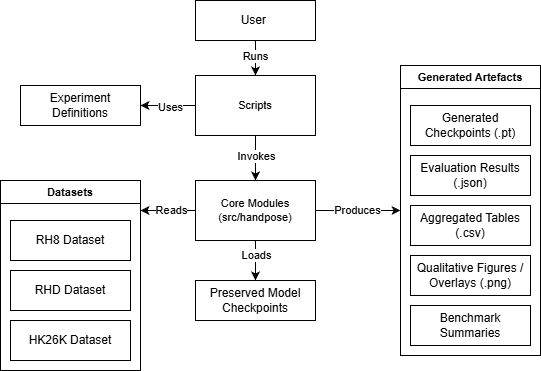
\includegraphics[width=0.7\textwidth]{4006_software_report-Page-2.drawio.png}
\caption{High-level architecture.}
\label{fig:software-architecture}
\end{figure}

\begin{figure}[htbp]
\centering
\begin{minipage}[t]{0.8\textwidth}
\centering
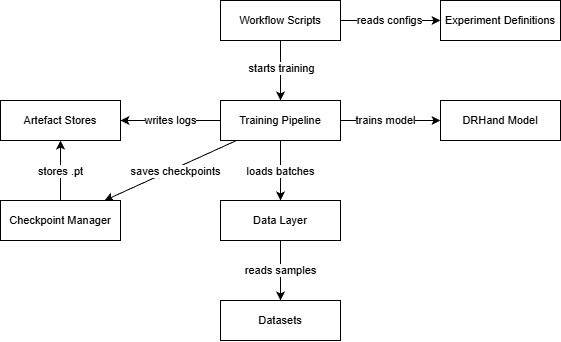
\includegraphics[width=\linewidth]{4006_software_report-comp_train_view.drawio.png}
\end{minipage}
\hfill
\begin{minipage}[t]{0.7\textwidth}
\centering
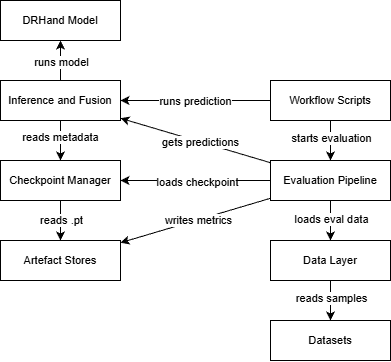
\includegraphics[width=\linewidth]{4006_software_report-comp_eval_view .drawio.png}
\end{minipage}
\caption{Training and evaluation component views.}
\label{fig:training-evaluation-component-views}
\end{figure}

\begin{figure}[htbp]
\centering
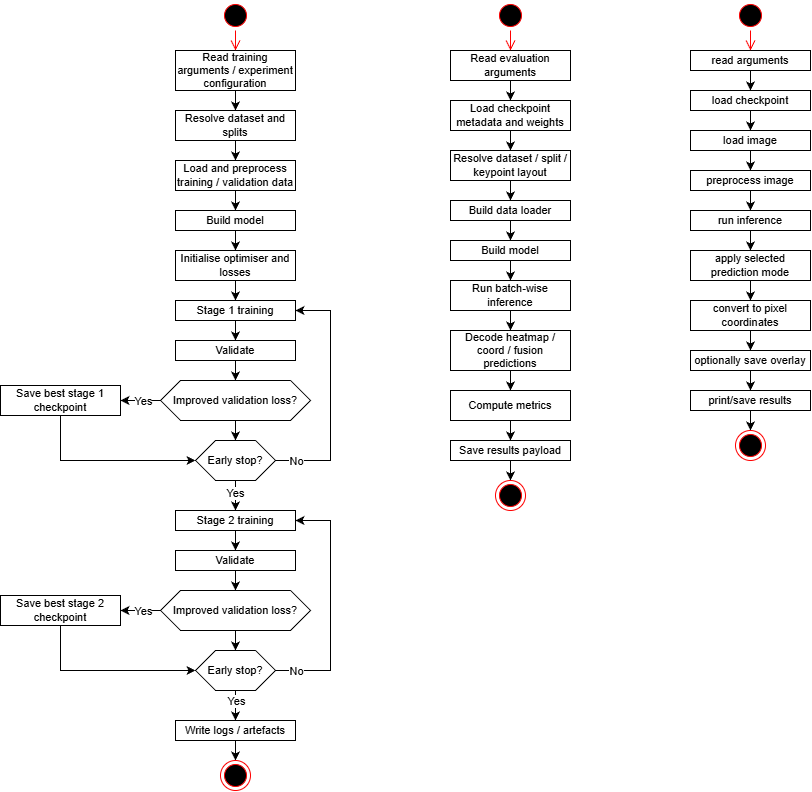
\includegraphics[width=1\textwidth,height=0.7\textheight,keepaspectratio]{4006_software_report-Page-4.drawio.png}
\caption{Training, evaluation and inference activity diagrams.}
\label{fig:training-evaluation-activities}
\end{figure}

\subsubsection*{Overall Structure}

Figure~\ref{fig:software-architecture} shows the overall system structure. The
repository is designed as a modular research artefact in which thin
command-line scripts provide the user-facing workflows, while the reusable
implementation is contained in the \path{src/handpose/} package. This
separates workflow orchestration from the core hand-pose logic and allows the
same internal code to support training, evaluation, benchmarking, and
single-image inference.

\medskip

At the highest level, the user interacts with the software by running scripts
such as \path{scripts/train.py}, \path{scripts/eval_metrics.py}, and
\path{scripts/predict_image.py}. These scripts optionally use experiment
definitions and generated command files, then invoke the core modules
responsible for data loading, model execution, training, inference, evaluation,
and checkpoint handling.

\medskip

The core modules read dataset files from disk and produce new artefacts such as
trained checkpoints, evaluation JSON files, aggregated CSV tables, benchmark
summaries, and qualitative figures. This structure keeps the execution
interface simple while ensuring that the main implementation remains reusable
and consistent across workflows.

\subsubsection*{Training View}

Figure~\ref{fig:training-evaluation-component-views} expands this design into
separate training and evaluation component views. In the training view, the
workflow scripts start the training pipeline, which requests batches from the
data layer, passes them through the DRHand model, computes the required losses,
and updates the model parameters.

\medskip

The data layer provides a shared interface for loading and preprocessing
supported datasets into normalized tensor representations. During training, the
checkpoint manager validates and saves model state together with metadata,
while the training pipeline also writes logs and loss histories to the
artefact store.

\subsubsection*{Evaluation and Inference View}

In the evaluation and inference view, the workflow scripts start either
checkpoint evaluation or direct prediction. The evaluation pipeline loads a
saved checkpoint through the checkpoint manager, rebuilds the model
configuration, obtains evaluation samples from the data layer, and requests
predictions from the inference and fusion module.

\medskip

That module runs the DRHand model, decodes heatmap outputs, uses the
coordinate branch predictions, and applies the fusion rule when fused
inference is requested.

\medskip

The resulting predictions are then used by the evaluation pipeline to compute
metrics such as SSE, EPE, PCK, timing information, and optional fusion
diagnostics, which are written back to the artefact store as structured
outputs.

\subsubsection*{Workflow Activities}

Figure~\ref{fig:training-evaluation-activities} complements the component
views by showing the workflows as activities.
It emphasizes the execution order of the main repository tasks: training moves
from dataset loading and preprocessing to staged optimisation, validation, and
checkpoint export, while evaluation and inference move from checkpoint loading
and sample preparation to prediction, fusion, metric computation, and output
generation.

\subsubsection*{Interfaces Between Components}

The interfaces between these components are mainly file-based and tensor-based.
File-based interfaces include dataset roots, annotation files, checkpoint
\texttt{.pt} files, evaluation \texttt{.json} outputs, summary \texttt{.csv}
files, and rendered \texttt{.png} figures.

\medskip

In-memory interfaces are primarily PyTorch tensors representing images,
keypoint coordinates, visibility values, heatmaps, and predicted coordinates.
Checkpoint metadata provides an additional interface between workflows by
preserving information such as training stage, epoch, keypoint layout, and
other configuration details needed to reload and evaluate a model correctly.

\subsection{Data Model(s), Including In-Memory Structures and Persistent Storage}

\subsubsection*{Processed Data}

The main inputs are RGB hand images and per-image
annotations from the supported datasets, including 2D keypoint coordinates and
visibility values. During preprocessing, these inputs are converted into a
shared tensor representation that is reused across training, evaluation, and
inference.

\subsubsection*{In-Memory Representation}

The main in-memory structures are image tensors of shape \texttt{(C,H,W)},
keypoint-coordinate tensors of shape \texttt{(K,2)}, visibility tensors of
shape \texttt{(K)}, predicted heatmaps of shape \texttt{(K,64,64)}, and
predicted coordinate tensors of shape \texttt{(K,2)}.

Where C denotes the number of image channels, H and W denote image height and
width, K denotes the number of keypoints, and N denotes batch size. The model
uses RGB inputs, so typically C = 3, and the predicted heatmaps have spatial
size 64 x 64.

\subsubsection*{Persistent Storage}

Persistent storage in the repository is file-based. Source datasets remain on
disk as image and annotation files, while intermediate and final outputs are
saved as experiment artefacts. Training checkpoints are written as PyTorch
\texttt{.pt} files containing model state and metadata, loss histories are
stored as CSV, evaluation outputs are written as JSON, aggregated summaries are
stored as CSV, and qualitative overlays or rendered figures are exported as
\texttt{.png}.
This design supports reproducibility because trained states, metrics, and
generated figures can all be reloaded or compared directly from the
filesystem.

\medskip

\begin{table}[htbp]
\centering
\small
\begin{tabular}{|p{0.22\textwidth}|p{0.34\textwidth}|p{0.22\textwidth}|}
\hline
\textbf{Data item} & \textbf{In-memory form} & \textbf{Persistent form} \\
\hline
RGB input image & Preprocessed tensor \texttt{(3,H,W)} & \texttt{.png} or \texttt{.jpg} image files \\
\hline
Ground-truth hand pose & Keypoint tensor \texttt{(K,2)} plus visibility tensor \texttt{(K)} & RHD annotations or COCO-style \texttt{.json} annotations \\
\hline
Training / evaluation batch & Batched tensors such as \texttt{(N,3,H,W)} and \texttt{(N,K,2)} & Runtime only; constructed by data loaders \\
\hline
Model predictions & Heatmaps \texttt{(N,K,64,64)} and coordinates \texttt{(N,K,2)} & Exported prediction or metric payloads in \texttt{.json}; optional qualitative \texttt{.png} outputs \\
\hline
Checkpoint state & Python dict containing \texttt{model\_state}, keypoint layout, stage, epoch, and training metadata & PyTorch checkpoint \texttt{.pt} files \\
\hline
Result summaries & Scalar metrics and aggregated experiment statistics & CSV tables and JSON result files \\
\hline
\end{tabular}
\caption{Main data representations used by the repository.}
\label{tab:data-representations}
\end{table}

\subsection{Significant Methods, Functions, or Other Lower-Level Elements}

\subsubsection*{Core Model}

The most important lower-level implementation element is \texttt{HandPoseNet}
in \path{src/handpose/models/hand_pose_model.py}, which acts as the main
wrapper around the learned model.

\medskip

It combines the shared backbone, heatmap regression head, and coordinate
regression head into one interface and provides the forward paths used during
both training and inference. This makes it the central model component on
which the rest of the repository depends.

\subsubsection*{Architecture and Optimisation}

At the architectural level, the most significant lower-level classes are
\texttt{Backbone}, \texttt{Heatmap\_reg}, and \texttt{coord\_reg} in
\path{src/handpose/models/architecture.py}, together with the reusable block
definitions in \path{src/handpose/models/block.py}.

\medskip

These classes implement the shared feature extractor, the heatmap branch, the
coordinate branch, and the depthwise-separable and upsampling building blocks
from which the DRHand-inspired model is assembled.

\medskip

The most important optimisation-related functions are
\texttt{coords\_to\_heatmaps}, \texttt{HeatmapMSELoss}, and \texttt{WingLoss}
in \path{src/handpose/models/losses.py}, along with
\texttt{build\_optimizer\_stage1}, \texttt{build\_optimizer\_stage2},
\texttt{train\_one\_epoch}, and \texttt{validate} in the training modules.

These functions define how supervision targets are constructed, how the two
training losses are computed, how different stages of the model are optimised,
and how batch-wise training and validation are carried out.

\subsubsection*{Data Processing and Fusion}

Another important group of lower-level functions appears in the preprocessing
and dataset-loading code. The dataset factory and dataset classes in
\path{src/handpose/data/} provide a unified interface for loading RHD and
COCO-style hand datasets, while preprocessing helpers in
\path{src/handpose/data/transforms.py} resize images, convert them to
tensors, and rescale keypoint coordinates.
These functions are significant because all training, evaluation, and
inference workflows depend on the same shared input format.

\medskip

The lower-level functions implementing branch fusion. 
In \path{src/handpose/inference/fusion.py}, functions such as
\texttt{heatmaps\_to\_coords\_argmax}, \texttt{resolve\_fusion\_bone\_edges},
and \texttt{fuse\_coords} define how heatmap predictions are decoded and how
the final fused prediction is selected from the heatmap and coordinate
branches.
These functions are central because the fusion rule is one of the defining
design features of the implemented pipeline.

\subsubsection*{Checkpointing and Workflow Entry Points}

Checkpoint and evaluation handling. 
Functions in \path{src/handpose/checkpoints.py} define how
checkpoints are validated, saved, and reloaded, while
\texttt{evaluate\_checkpoint} in
\path{src/handpose/evaluation/eval_metrics_core.py} performs the main
metric computation for SSE, EPE, PCK, timing, and optional fusion diagnostics.
These components are important because they make the repository reproducible
and allow trained models to be reused consistently across training, inference,
and result generation workflows.

\medskip

The user-facing scripts under \path{scripts/} are thin but
important workflow connectors. Scripts such as \texttt{train.py},
\path{eval_metrics.py}, \path{predict_image.py}, and
\path{benchmark_pipeline.py} do not contain the main modelling logic
themselves, but they are the main entry points through which a user accesses
the lower-level implementation for complete training, evaluation, inference,
and benchmarking tasks.

\subsection{Important Errors and Their Conditions}

\subsubsection*{Input and Configuration Errors}

Several important errors in the software are caused by invalid inputs, missing
files, or inconsistent configuration between artefacts. For example, the
checkpoint utilities raise errors when a checkpoint is missing required
metadata fields, has a mismatched keypoint layout, contains duplicate keypoint
indices, or uses an unsupported checkpoint version. Similar validation errors
occur when invalid keypoint subsets are requested, when unsupported dataset
names or split aliases are supplied, or when an invalid prediction mode or
negative PCK threshold is passed on the command line.
In these cases, the software responds by raising a clear \texttt{ValueError}
and stopping execution rather than continuing with inconsistent state.

\subsubsection*{Runtime Resource Errors}

A second group of important errors occurs when required runtime resources are
not available. Examples include missing dataset directories, missing image
files, empty evaluation image folders, failed imports of optional dependencies
such as MediaPipe, or requesting CUDA on a machine where it is not available.
These conditions are handled through exceptions such as
\texttt{FileNotFoundError} or \texttt{RuntimeError}.
The software does not silently ignore these problems; instead, it fails early
and reports the missing dependency, missing path, or unsupported device
condition so that the user can correct the environment before rerunning the
workflow.

\subsubsection*{Workflow State Errors}

Further errors can arise from invalid workflow state during training or
evaluation. For example, stage-specific training functions raise errors if an
unsupported stage number is used, if gradient accumulation is configured with
an invalid value, or if stage 2 is requested without the required coordinate
loss. Training also raises an error if \texttt{--skip-stage1} is used without
providing an initial checkpoint.

\medskip

Evaluation and qualitative-rendering workflows can also fail when no samples
match the requested dataset split or when the selected checkpoint does not
contain the keypoints required for shared-10 evaluation or fusion. In these
situations, the software again responds by terminating with an explicit error
message, which helps prevent silent misuse of the repository and makes
debugging more straightforward.

\subsection{User Interface Design}

\subsubsection*{Command-Line Interaction}

The user interacts with the software primarily through a command-line
interface. The main workflows are exposed as separate Python scripts under
\path{scripts/}, including training, evaluation, benchmarking,
single-image inference, qualitative rendering, and result aggregation.

\medskip

In practice, the user runs these scripts from the repository root, supplies
the required paths and options as command-line arguments, and receives outputs
such as checkpoints, JSON result files, CSV summaries, printed metrics, or
rendered visualisations.

\medskip

This command-line design was chosen because the software is a research
artefact rather than an end-user application. The main tasks involve running
controlled experiments, reproducing reported results, evaluating checkpoints
under different conditions, and generating analysis artefacts.

\medskip

These activities are better supported by explicit script arguments than by a
graphical user interface, because command-line workflows are easier to
document, automate, reproduce, and integrate with local machines, Conda
environments, and HPC or Slurm-based execution.

\subsubsection*{Separation of Interface and Core Logic}

Another important interface choice was to separate the reusable implementation
from the user-facing entry points. The core logic is implemented in the
\path{src/handpose/} package, while the scripts act as thin workflow
wrappers around that logic.
This was done so that the user interface remains simple at the script level
while the lower-level code remains modular and reusable. As a result, users
can run complete workflows through a small number of documented commands
without needing to interact directly with the internal package structure.

\subsubsection*{Explicit Runtime Configuration}

The interface relies on explicit file and path arguments for datasets,
checkpoints, and output locations. This choice was made to keep the repository
portable across different machines and storage layouts, especially since some
datasets are external and not bundled with the artefact.
By making these dependencies explicit at runtime, the software avoids
hard-coding machine-specific paths and makes the execution process clearer for
assessors and future users.

\subsection{Quality Assurance Steps}

\subsubsection*{Documentation and Artefact Management}

Maintainability was further supported through reproducibility-oriented
documentation and artefact management. The repository includes installation
instructions, requirement notes, a replication guide, curated experiment
command files, preserved checkpoints, and saved result artefacts.
These were important quality-assurance measures because they made the software
easier to inspect, rerun, and extend, while also ensuring that the reported
experimental outputs could be traced back to concrete workflows within the
repository.

\subsubsection{Version Control and Versioning}

Version control was used throughout development by maintaining the project as a
Git-based repository. This allowed the software, documentation, experiment
definitions, and preserved artefacts to be developed within a single
structured history rather than as disconnected files.
Using version control was important because the project involved repeated
changes to model design, training configuration, evaluation workflows,
reporting artefacts, and supporting documentation, all of which needed to
remain traceable over time.

\medskip

Changes were tracked and managed through the normal Git workflow of recording
edits to the repository as development progressed. This made it possible to
monitor the evolution of scripts, source modules, experiment files, and paper
materials, and helped prevent important changes from being lost or mixed
together without record.
It also supported safer experimentation, since alternative implementations or
revised configurations could be introduced while preserving the earlier state
of the project.

\subsubsection{Code Style and Convention}

The code follows a consistent Python style based on clear module separation,
descriptive function names, and lightweight internal documentation. The
repository is organised by responsibility, with separate modules for data
loading, model definition, training, inference, evaluation, and checkpoint
handling.
Within these modules, functions and classes generally use descriptive
snake\_case naming for functions and variables, and class-based naming for
model components such as \texttt{HandPoseNet}. This made the code easier to
navigate because related logic was grouped together rather than scattered
across large scripts.

\medskip

A consistent convention was also followed for docstrings and purpose
statements. Most modules begin with a short summary docstring explaining their
role in the repository, and most important functions include concise
docstrings describing what they do.
This helped keep the code clear because users and future readers can
understand the role of a file or function without having to infer it entirely
from implementation details.

\medskip

The code also follows a convention of keeping user-facing workflow logic
separate from reusable implementation logic. Scripts under \path{scripts/}
mainly parse arguments and call functions from the \path{src/handpose/}
package, while the package itself contains the lower-level logic.
This convention improved consistency because training, evaluation, inference,
and benchmarking were all built on shared internal code rather than separate
duplicated implementations.

\medskip


The use of explicit validation and informative error 
messages at key interfaces. Functions that depend on specific
assumptions, such as checkpoint schema, prediction modes, dataset names,
keypoint layouts, or device availability, usually check these conditions
directly and raise clear exceptions if they are violated.
This kept the behaviour of the software more predictable and made the codebase
easier to maintain, since failures tended to occur close to the source of the
problem rather than emerging later as ambiguous downstream bugs.

\subsubsection{Automated Testing}

The repository includes a lightweight automated test suite implemented with
\texttt{pytest}. These tests provide a fast validation layer
before running more expensive workflows such as full training or dataset-based
evaluation.

\medskip

\texttt{test\_hand\_pose\_net\_output\_shapes} in
\path{tests/test_model_shapes.py}. This test instantiates
\texttt{HandPoseNet} for both the standard 21-keypoint layout and the reduced
10-keypoint layout, passes a dummy tensor of shape \texttt{(2,3,256,256)}
through the model, and checks that the outputs have shapes
\texttt{(2,K,64,64)} for heatmaps and \texttt{(2,K,2)} for coordinates. It
also checks that the returned tensors contain only finite values. This
verifies the most basic output-shape contract of the model.

\medskip

\texttt{test\_heatmaps\_to\_coords\_argmax\_decodes\_normalized\_xy} in
\path{tests/test_fusion.py}. This test constructs a small heatmap with a known
maximum location and checks that \texttt{heatmaps\_to\_coords\_argmax}
returns the expected normalized coordinate. The same file also includes
\texttt{test\_resolve\_fusion\_bone\_edges\_supports\_tip\_base\_10\_and\_rejects\_other\_layouts},
which checks that supported keypoint layouts are accepted while unsupported
layouts raise a \texttt{ValueError}. These tests verify both correct fusion
behaviour and correct rejection of invalid inputs.

\medskip

\texttt{test\_validate\_checkpoint\_accepts\_and\_normalizes\_valid\_schema} in
\path{tests/test_checkpoints.py}. This test supplies checkpoint metadata with
string values for stage and epoch and checks that validation normalizes them
correctly. The same file also includes
\texttt{test\_validate\_checkpoint\_rejects\_duplicate\_keypoint\_indices} and
\texttt{test\_validate\_checkpoint\_rejects\_inconsistent\_num\_keypoints},
which confirm that malformed checkpoint metadata is rejected. These tests
protect the checkpoint contract used by training, evaluation, and inference
workflows.

\end{document}


